%%%%%%%%%%%%%%%%%%%%%%%%%%%%%%%%%%%%%%%%%
% Friggeri Resume/CV
% XeLaTeX Template
% Version 1.0 (5/5/13)
%
% This template has been downloaded from:
% http://www.LaTeXTemplates.com
%
% Original author:
% Adrien Friggeri (adrien@friggeri.net)
% https://github.com/afriggeri/CV
%
% License:
% CC BY-NC-SA 3.0 (http://creativecommons.org/licenses/by-nc-sa/3.0/)
%
% Important notes:
% This template needs to be compiled with XeLaTeX and the bibliography, if used,
% needs to be compiled with biber rather than bibtex.
%
%%%%%%%%%%%%%%%%%%%%%%%%%%%%%%%%%%%%%%%%%

\documentclass[a4paper,latin]{friggeri-cv} % Add 'print' as an option into the square bracket to remove colors from this template for printing
\hypersetup{
pdftitle={Bewerbungsunterlagen von Sascha Manns}, %%
pdfauthor={Sascha Manns}, %%
pdfsubject={Bewerbungsunterlagen}, %%
pdfcreator={XeLaTEX and Biber with hyperref-package.},
pdfproducer={Sascha Manns, Mayen}, %%
pdfkeywords={Manns, Mayen, Bewerbung, IT, Community, Linux, Programmierer, Dispatcher, Buchautor, Schriftsteller, Geschäftsprozess} %%
}
\usepackage{pdfpages}
\usepackage{graphicx}
\usepackage{xltxtra}
\usepackage{progressbar}

\addbibresource{../Appendix/Bibliography/bibliography1.bib} % Specify the bibliography file to include publications

\begin{document}
%\includepdf{../Cover/Cover}

\header{Sascha}{Manns}{Supporter/Documentation Specialist} % Your name and current job title/field

%----------------------------------------------------------------------------------------
%	SIDEBAR SECTION
%----------------------------------------------------------------------------------------

\begin{aside} % In the aside, each new line forces a line break
\section{Kontakt}
Maifeldstraße 10
56727 Mayen
Germany
~
+49 (1573) 924 2730
+49 (2651) 40 14 045
~
\href{mailto:Sascha.Manns@directbox.com}{Sascha.Manns@directbox.com}
\includegraphics[width=0.3cm]{../Pictures/email.png}
\href{http://saigkill.github.io}{saigkill.github.io}
\includegraphics[width=0.3cm]{../Pictures/aboutme.png}
Geburtsdatum: 01.10.1979
\section{Social Media}
\href{https://www.xing.com/profile/Sascha\_Manns2}{Sascha\_Manns2}
\includegraphics[width=0.3cm]{../Pictures/xing.png}
\href{https://www.linkedin.com/in/saigkill}{saigkill}
\includegraphics[width=0.3cm]{../Pictures/linkedin.png}
\href{https://www.facebook.com/sascha.manns}{sascha.manns}
\includegraphics[width=0.3cm]{../Pictures/facebook.png}
\href{https://plus.google.com/+SaschaManns}{+SaschaManns}
\includegraphics[width=0.3cm]{../Pictures/google-plus.png}
\href{https://twitter.com/saigkill}{saigkill}
\includegraphics[width=0.3cm]{../Pictures/twitter.png}
%\href{https://coderbits.com/saigkill}{saigkill}
\includegraphics[width=0.3cm]{../Pictures/coderbits.png}
\section{Fremdsprachen}
Deutsch \progressbar[linecolor=blue,tickscolor=orange,emptycolor=white,filledcolor=blue]{1.0}
Englisch \progressbar[linecolor=blue,tickscolor=orange,emptycolor=white,filledcolor=blue]{0.6}
Russisch \progressbar[linecolor=blue,tickscolor=orange,emptycolor=white,filledcolor=blue]{0.3}
\section{Programming}
{Shell (Bash)}\progressbar[linecolor=blue,tickscolor=orange,emptycolor=white,filledcolor=green]{0.6}
{JavaScript}\progressbar[linecolor=blue,tickscolor=orange,emptycolor=white,filledcolor=green]{0.3}
{CSS \& HTML5}\progressbar[linecolor=blue,tickscolor=orange,emptycolor=white,filledcolor=green]{0.6}
{Ruby}\progressbar[linecolor=blue,tickscolor=orange,emptycolor=white,filledcolor=green]{0.7}
\end{aside}

%----------------------------------------------------------------------------------------
%	WORK EXPERIENCE SECTION
%----------------------------------------------------------------------------------------

\section{Berufserfahrung}

\begin{entrylist}
%------------------------------------------------
\entry{09/2015--jetzt}
{Myself}
{Homeoffice}
{\emph{Aktive Bewerbungsphase}
}
%------------------------------------------------
\entry{09/2014--09/2015}
{XCOM AG}
{Andernach}
{\emph{Documentation Specialist} \\
	Detailierte Aufgaben:
	\begin{itemize}
		\item Autor Geschäftsprozessdokumentation (Software \& Bankwesen)
		\item Artikelerstellung und Pflege internes Wiki
		\item Produktion Präsentationen für Mandanten und interne Schulungen
		\item Modellierung von Geschäftsprozessen nach BPMN
	\end{itemize}
	Vertragsauslauf aufgrund der Verschiebung der Stelle in eine andere Zweigstelle.
}
%------------------------------------------------
\entry
{02/2014--05/2014}
{Hays Temp GmbH / More Holding}
{Mannheim}
{\emph{IT-Supporter/Dispatcher/Controller} \\
Detailierte Aufgaben bei ITSCare Neuwied (ZBV):
\begin{itemize}
\item Kundenpflege via Telefon und Email
\item Dispatching und Teamcontroling
\item AmSys/IDM (AOK Krankenkassen)
\item Eröffnung, Entsperrung oder Löschung von Benutzerkonten
\item Passwort- und Rechtevergaben
\item SLA-konforme Bearbeitung von eingehenden Störungen (betreffend Benutzerverwaltung) im Rahmen des Incident-Managements
\item Pflege von Logon-Prozeduren
\item Annahme, Erfassung und Bearbeitung eingehender Benutzeranträge
\item Benutzerkontenverwaltung im Active Directory
\end{itemize}
}
%------------------------------------------------
\entry
{11/2012--10/2013}
{Lulu Press Inc.}
{Homeoffice}
{\emph{Buchautor \& Herausgeber}\\
Detailierte Aufgaben:
\begin{itemize}
\item Recherche
\item Schreiben des Handbuchs
\item Einführung des Lektorenteams in das Projekt
\item Einführung einer Google Code-In Studentin in den Textsatz (Teilnahme als Mentor)
\item Satz \& Layout (\LaTeX{} und DocBook/XSL-FO)
\end{itemize}
}
%------------------------------------------------
\entry
{08/2010--06/2013}
{open-slx GmbH}
{Homeoffice}
{\emph{Community \& Support Agent} \\
Detailierte Aufgaben:
\begin{itemize}
\item Level 1 \& 2 Support via Telefon und Email
\item Testen von Software
\item Webseitenbetreuung \& Social Media
\item Dokumentation
\item Community Management
\item Projektleitung deutsches openSUSE Wiki. Migration des Wikis zu neuer Struktur
\item openSUSE Weekly News
\item Paketverwaltung einiger RPM-Pakete
\item openSUSE Membership Application Team
\end{itemize}
Auflösung der Stelle durch mangelnde Absatzzahlen des Boxproduktes.
}
\end{entrylist}
\begin{entrylist}
%------------------------------------------------
\entry
{07/2007--12/2014}
{openSUSE Linux Projekt}
{Homeoffice}
{\emph{Paketbetreuer/Teamleiter}\\
Detailierte Aufgaben:
\begin{itemize}
\item Beschaffung, Aktualisierung des Sourcecodes im Buildservice
\item Compiling und Packaging neuer Binärpakete
\item Verteilung via Buildservice
\item Leiter des openSUSE Newsletters und Publikationen in bis zu 12 Sprachen
\item Erfinder eines neuen Podcastformates (Vertonte Weekly News)
\item openSUSE Medical Project (Subprojektgründer)
\item Mitglied des openSUSE Marketing Teams
\item Mitglied des openSUSE Feature Screening Teams
\end{itemize}
}
%-----------------------------------------------
\entry
{07/2000--06/2007}
{Geistlicher eines religiösen Ordens}
{Selters/Ts.}
{\emph{Ersatzdienst zum Zivildienst}}
\end{entrylist}
\begin{entrylist}
%------------------------------------------------
\entry
{08/1998--07/2000}
{Auto Deschner GmbH}
{Mendig}
{\emph{Kaufmann im Einzelhandel}\\
Detailierte Aufgaben:
\begin{itemize}
\item Einkauf \& Warenannahme \& Kontrolle
\item Bestandsbuchungen der Waren
\item Kundenbetreuung
\item Rechnungserstellung
\item Projektplanung
\end{itemize}
}
\end{entrylist}

\section{Berufsausbildung}
\begin{entrylist}
%------------------------------------------------
\entry
{08/1995--08/1998}
{Auto Deschner GmbH}
{Mendig}
{\emph{Ausbildung zum Kaufmann im Einzelhandel}\\
Allgemeine kaufm. Tätigkeiten.
}
%------------------------------------------------
\end{entrylist}

%----------------------------------------------------------------------------------------
%	EDUCATION SECTION
%----------------------------------------------------------------------------------------

\section{Weiterbildung \& Zertifikate}

\begin{entrylist}
%------------------------------------------------
\entry
{06/2015}
{SCRUM Master Kurs}
{XCOM AG, Inhouse Schulung}
{Andernach}
%------------------------------------------------
\entry
{12/2013}
{Web Engeneering 1}
{Technische Hochschule Mittelhessen}
{\emph{MOOC}}
%------------------------------------------------
%\entry
%{06/2013}
%{Kompetenzpass für Ökonomen}
%{BV Deutscher Volks- und Betriebswirte}
%{Düsseldorf}
%------------------------------------------------
\entry
{04/2013}
{Onlinequalifizierung: Schlüsselkompetenzen kompakt}
{Career Webinars}
{Web}
%-----------------------------------------------
\end{entrylist}

%----------------------------------------------------------------------------------------
%	EHRENAMTLICHE TÄTIGKEITEN
%----------------------------------------------------------------------------------------
\section{Ehrenamtliche Tätigkeiten}
\begin{entrylist}
%--------------------------------------------
\entry
{2013-jetzt}
{mUXCamp}
{mUXCamp, Worms}
{Planungsteam für nächstes Camp. (Mitveranstalter: \\FG Wirtschaftsinformatik des BDVB)}
%--------------------------------------------
%\entry
%{2013--jetzt}
%{BV Deutscher Volks- und Betriebswirte}
%{FG Wirtschaftsinformatik}
%{Mitarbeit in verschiedenen Projekten}
%---------------------------------------------
\entry
{2010--2011}
{Piratenpartei Deutschland}
{Bundespressestelle}
{}
%--------------------------------------------
\entry
{2008--2015}
{openSUSE Linux Project}
{Membership Application Team/RPM Packaging}
{Mitgliederverwaltung \& Paketverwaltung}
%--------------------------------------------
\end{entrylist}

\newpage
%----------------------------------------------------------------------------------------
% COMPUTER SKILLS
% ---------------------------------------------------------------------------------------

\section{IT-Kenntnisse}

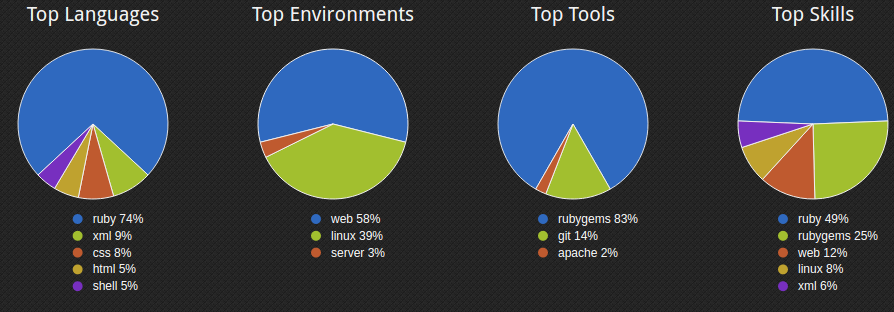
\includegraphics[width=13cm]{../Pictures/Skills1.png} \linebreak
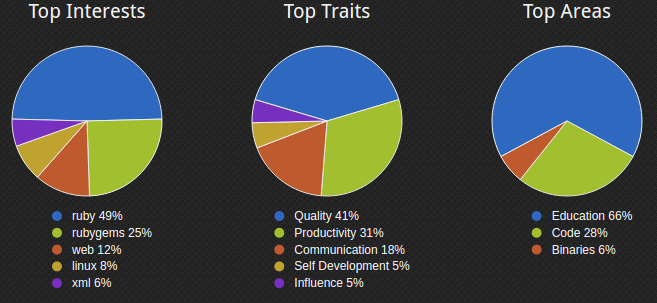
\includegraphics[width=13cm]{../Pictures/Skills2.png}

\begin{itemize}
\item Operating Systems:
    \begin{itemize}
      \item Linux/Unix \hfill \progressbar[linecolor=blue,tickscolor=orange,emptycolor=white,filledcolor=red ]{0.8} \hfill
      \item Windows 3.11--8.1 \hfill \progressbar[linecolor=blue,tickscolor=orange,emptycolor=white,filledcolor=red ]{0.7} \hfill
    \end{itemize}
\item ERM/CRM:
    \begin{itemize}
      \item ADP Opel Verkäuferarbeitsplatz \hfill \progressbar[linecolor=blue,tickscolor=orange,emptycolor=white,filledcolor=red ]{0.2} \hfill
      \item Warenwirtschaftssysteme \hfill \progressbar[linecolor=blue,tickscolor=orange,emptycolor=white,filledcolor=red ]{0.4} \hfill
      \item oscare (SAP Lösung für Gesundheitsbranche) \hfill \progressbar[linecolor=blue,tickscolor=orange,emptycolor=white,filledcolor=red ]{0.7} \hfill
    \end{itemize}
\item Linux-Software-Packaging:
    \begin{itemize}
      \item RPM-Pakete \hfill \progressbar[linecolor=blue,tickscolor=orange,emptycolor=white,filledcolor=red ]{0.6} \hfill
      \item DEB-Pakete \hfill \progressbar[linecolor=blue,tickscolor=orange,emptycolor=white,filledcolor=red ]{0.8} \hfill
      \item Compiling/Testing/Publishing \hfill \progressbar[linecolor=blue,tickscolor=orange,emptycolor=white,filledcolor=red ]{0.8} \hfill
      \item Git/SVN \hfill \progressbar[linecolor=blue,tickscolor=orange,emptycolor=white,filledcolor=red ]{0.8} \hfill
      \item OTRS \hfill \progressbar[linecolor=blue,tickscolor=orange,emptycolor=white,filledcolor=red ]{0.8} \hfill
    \end{itemize}
\item Textsatz:
    \begin{itemize}
      \item \LaTeX \hfill \progressbar[linecolor=blue,tickscolor=orange,emptycolor=white,filledcolor=red ]{0.7} \hfill
      \item Docbook 4.5/5 \& XSL-FO \hfill \progressbar[linecolor=blue,tickscolor=orange,emptycolor=white,filledcolor=red ]{0.8} \hfill
    \end{itemize}
\item Administration: Linux/Unix \hfill\progressbar[linecolor=blue,tickscolor=orange,emptycolor=white,filledcolor=red ]{0.7}\hfill
\item Webservices:
    \begin{itemize}
      \item Apache2 \hfill \progressbar[linecolor=blue,tickscolor=orange,emptycolor=white,filledcolor=red ]{0.6}\hfill
      \item Joomla \hfill \progressbar[linecolor=blue,tickscolor=orange,emptycolor=white,filledcolor=red ]{0.6} \hfill
      \item Owncloud \hfill \progressbar[linecolor=blue,tickscolor=orange,emptycolor=white,filledcolor=red ]{0.7} \hfill
      \item Wordpress \hfill \progressbar[linecolor=blue,tickscolor=orange,emptycolor=white,filledcolor=red ]{0.7} \hfill
    \end{itemize}
\item Multimedia:
    \begin{itemize}
      \item Pod- \& Screencastproduktion \hfill \progressbar[linecolor=blue,tickscolor=orange,emptycolor=white,filledcolor=red ]{0.8} \hfill
      \item Videoschnitt \hfill \progressbar[linecolor=blue,tickscolor=orange,emptycolor=white,filledcolor=red ]{0.6} \hfill
    \end{itemize}
\item Office:
    \begin{itemize}
      \item MS-Office \hfill \progressbar[linecolor=blue,tickscolor=orange,emptycolor=white,filledcolor=red ]{0.6} \hfill
      \item LibreOffice \hfill \progressbar[linecolor=blue,tickscolor=orange,emptycolor=white,filledcolor=red ]{0.7} \hfill
      \item SoftMaker-Office \hfill \progressbar[linecolor=blue,tickscolor=orange,emptycolor=white,filledcolor=red ]{0.7} \hfill
      \item Projektmanagement-Software \hfill \progressbar[linecolor=blue,tickscolor=orange,emptycolor=white,filledcolor=red ]{0.7} \hfill
    \end{itemize}
\item Produktgestaltung:
    \begin{itemize}
      \item Handbucherstellung \hfill \progressbar[linecolor=blue,tickscolor=orange,emptycolor=white,filledcolor=red ]{0.9} \hfill
      \item Supportdatenbank \hfill \progressbar[linecolor=blue,tickscolor=orange,emptycolor=white,filledcolor=red ]{0.8} \hfill
      \item Webpräsentation \hfill \progressbar[linecolor=blue,tickscolor=orange,emptycolor=white,filledcolor=red ]{0.7} \hfill
    \end{itemize}
\item Wissensmanagement:
    \begin{itemize}
      \item MS Sharepoint \hfill \progressbar[linecolor=blue,tickscolor=orange,emptycolor=white,filledcolor=red ]{0.5} \hfill
      \item Business Wiki \hfill \progressbar[linecolor=blue,tickscolor=orange,emptycolor=white,filledcolor=red ]{0.7} \hfill
      \item Business Social Networks \hfill \progressbar[linecolor=blue,tickscolor=orange,emptycolor=white,filledcolor=red ]{0.7} \hfill
    \end{itemize}
\item IDE's:
    \begin{itemize}
      \item Visual Studio \hfill \progressbar[linecolor=blue,tickscolor=orange,emptycolor=white,filledcolor=red ]{0.5} \hfill
      \item RubyMine/IntelliJ \hfill \progressbar[linecolor=blue,tickscolor=orange,emptycolor=white,filledcolor=red ]{0.8} \hfill
      \item Oxygen-XML-Editor \hfill \progressbar[linecolor=blue,tickscolor=orange,emptycolor=white,filledcolor=red ]{0.8} \hfill
    \end{itemize}
\end{itemize}

%----------------------------------------------------------------------------------------
%	COMMUNICATION SKILLS SECTION
%----------------------------------------------------------------------------------------

\section{Kommunikation}

\begin{entrylist}
%------------------------------------------------
\entry
{2013}
{mUXCamp Worms}
{Standbetreuung}
{Vertretung der FG Wirtschaftsinformatik des BDVB}
%------------------------------------------------
\entry
{2010}
{openSUSE Conference}
{Vortrag}
{Vortrag über den aktuellen Stand der Weekly News und die Planungen der Zukunft}
%------------------------------------------------
\entry
{2010}
{openSUSE Conference}
{Vortrag}
{Vortrag über Open Source im Alltag}
%------------------------------------------------
\end{entrylist}

%----------------------------------------------------------------------------------------
%	INTERESTS SECTION
%----------------------------------------------------------------------------------------

\section{Interessen}

\includegraphics[width=13cm]{../Pictures/Interessen.png}

%----------------------------------------------------------------------------------------
%	PUBLICATIONS SECTION
%----------------------------------------------------------------------------------------
\newpage
\section{Publikationen}

\printbibsection{article}{Artikel} % Print all articles from the bibliography

\printbibsection{book}{Bücher} % Print all books from the bibliography

\begin{refsection} % This is a custom heading for those references marked as "inproceedings" but not containing "keyword=france"
\nocite{*}
\printbibliography[sorting=chronological, type=inproceedings, title={international peer-reviewed conferences/proceedings}, notkeyword={france}, heading=subbibliography]
\end{refsection}

\begin{refsection} % This is a custom heading for those references marked as "inproceedings" and containing "keyword=france"
\nocite{*}
\printbibliography[sorting=chronological, type=inproceedings, title={local peer-reviewed conferences/proceedings}, keyword={france}, heading=subbibliography]
\end{refsection}

\printbibsection{misc}{other publications} % Print all miscellaneous entries from the bibliography

\printbibsection{report}{research reports} % Print all research reports from the bibliography

%----------------------------------------------------------------------------------------

\begin{center}
\includegraphics[scale=0.7]{../Pictures/signatur.png} \\
\begin{tabular}{@{}l@{}}
\\ $\frac{}{\strut\textnormal{Sascha Manns, Mayen den \today}}$
\end{tabular}
\end{center}

%\section{Anhang}
%---------------------------------------------------------------------------

\end{document}
